%%%%%%%%%%%%%%%%%%%%%%%%%%%%%%%%%%%%

\section{Inference for a single proportion}

%%%%%%%%%%%%%%%%%%%%%%%%%%%%%%%%%%%%

\begin{frame}

\pq{Two scientists want to know if a certain drug is effective against high blood pressure. The first scientist wants to give the drug to 1000 people with high blood pressure and see how many of them experience lower blood pressure levels. The second scientist wants to give the drug to 500 people with high blood pressure, and not give the drug to another 500 people with high blood pressure, and see how many in both groups experience lower blood pressure levels. Which is the better way to test this drug?}

\begin{enumerate}[(a)]
\item All 1000 get the drug
\solnMult{500 get the drug, 500 don't}
\end{enumerate}

\end{frame}

%%%%%%%%%%%%%%%%%%%%%%%%%%%%%%%%%%%%

\begin{frame}
\frametitle{Results from the GSS}

The GSS asks the same question, below is the distribution of responses from the 2010 survey: \\

\begin{center}
\begin{tabular}{l c}
All 1000 get the drug		& 99 \\
500 get the drug 500 don't	& 571 \\
\hline
Total						& 670
\end{tabular}
\end{center}

\end{frame}

%%%%%%%%%%%%%%%%%%%%%%%%%%%%%%%%%%%

\begin{frame}
\frametitle{Parameter and point estimate}

\dq{We would like to estimate the proportion of all Americans who have good intuition about experimental design, i.e. would answer ``500 get the drug 500 don't"? What are the parameter of interest and the point estimate?}

\pause

\begin{itemize}

\item \hl{Parameter of interest:} Proportion of \orange{all} Americans who have good intuition about experimental design.
\[ \mathhl{p}~\scriptsize{(\text{a population proportion})} \]

\pause

\item \hl{Point estimate:} Proportion of \orange{sampled} Americans who have good intuition about experimental design.
\[ \mathhl{\hat{p}}~\scriptsize{(\text{a sample proportion})} \]

\end{itemize}

\end{frame}

%%%%%%%%%%%%%%%%%%%%%%%%%%%%%%%%%%%

\begin{frame}
\frametitle{Inference on a proportion}

\dq{What percent of all Americans have good intuition about experimental design, i.e. would answer ``500 get the drug 500 don't"?}

\pause

\begin{itemize}

\item We can answer this research question using a confidence interval, which we know is always of the form

\[ \textcolor{orange}{point~estimate \pm ME} \]

\pause

\item And we also know that \textcolor{orange}{$ME = critical~value \times standard~error$} of the point estimate.

\end{itemize}

\pause

\formula{Standard error of a sample proportion}
{
\[ SE_{\hat{p}} =  \sqrt{\frac{p~(1-p)}{n}}  \]
}


\end{frame}

%%%%%%%%%%%%%%%%%%%%%%%%%%%%%%%%%%%

\subsection{Identifying when a sample proportion is nearly normal}

%%%%%%%%%%%%%%%%%%%%%%%%%%%%%%%%%%%%

\begin{frame}
\frametitle{Sample proportions are also nearly normally distributed}

\formula{Central limit theorem for proportions}
{
Sample proportions will be nearly normally distributed with mean equal to the population mean, $p$, and standard error equal to $\sqrt{\frac{p~(1-p)}{n}}$.
\[ \hat{p} \sim N \pr{ mean = p, SE = \sqrt{\frac{p~(1-p)}{n}} } \]
}

But of course this is true only under certain conditions...

\dq{Any guesses?}

\soln{\pause{Independent observations, at least 10 successes and 10 failures}}

\pause

\Note{If $p$ is unknown (most cases), we use $\hat{p}$ in the calculation of the standard error.}

\end{frame}

%%%%%%%%%%%%%%%%%%%%%%%%%%%%%%%%%%%

%\begin{frame}
%\frametitle{A quick activity}
%
%\pq{Flip a coin 20 times -- this is going to get loud! Record the number of heads and then use your clicker to submit the proportion of heads you obtained.}
%
%\begin{enumerate}[(a)]
%\item $\le$ 0.3
%\item 0.4
%\item 0.5
%\item 0.6
%\item $\ge$ 0.7
%\end{enumerate}
%
%\end{frame}
%
%%%%%%%%%%%%%%%%%%%%%%%%%%%%%%%%%%%%

%\begin{frame}
%
%\formula{Central limit theorem for proportions}
%{
%Sample proportions will be nearly normally distributed with mean equal to the population mean, $p$, and standard error equal to $\sqrt{\frac{p~(1-p)}{n}}$.
%\[ \hat{p} \sim N \pr{ mean = p, SE = \sqrt{\frac{p~(1-p)}{n}} } \]
%If the population proportion is not available, use the sample proportion to estimate the standard error.
%}
%
%\pause
%
%Assumptions/conditions:
%\begin{enumerate}[1.]
%\item \hl{Independence}: 
%\begin{itemize}
%\item \hlGr{Random sample}
%\item \hlGr{10\% condition}: If sampling without replacement, $n <$ 10\% of the population.
%\end{itemize}
%\item \hl{Normality}: At least 10 successes and 10 failures.
%\end{enumerate}
%
%\end{frame}
%
%%%%%%%%%%%%%%%%%%%%%%%%%%%%%%%%%%%%

\subsection{Confidence intervals for a proportion}

%%%%%%%%%%%%%%%%%%%%%%%%%%%%%%%%%%%%

\begin{frame}
\frametitle{Back to experimental design...}

\dq{The GSS found that 571 out of 670 (85\%) of Americans answered the question on experimental design correctly. Estimate (using a 95\% confidence interval) the proportion of all Americans who have good intuition about experimental design?}

\pause
Given: $n = 670, \hat{p} = 0.85$. First check conditions.

\pause
\begin{enumerate}[1.]
\item \hl{Independence}: The sample is random, and 670 $<$ 10\% of all Americans, therefore we can assume that one respondent's response is independent of another.
\pause
\item \hl{Success-failure}: 571 people answered correctly (successes) and 99 answered incorrectly (failures), both are greater than 10.
\end{enumerate}

\end{frame}

%%%%%%%%%%%%%%%%%%%%%%%%%%%%%%%%%%%

\begin{frame}

\pq{We are given that  $n = 670, \hat{p} = 0.85$, we also just learned that the standard error of the sample proportion is $SE = \sqrt{\frac{p(1-p)}{n}}$. Which of the below is the correct calculation of the 95\% confidence interval?}

\begin{enumerate}[(a)]
\solnMult{$0.85 \pm 1.96 \times \sqrt{\frac{0.85 \times 0.15}{670}}$} \soln{\only<2>{\orange{$\rightarrow (0.82, 0.88)$}}}
\item $0.85 \pm 1.65 \times \sqrt{\frac{0.85 \times 0.15}{670}}$
\item $0.85 \pm 1.96 \times \frac{0.85 \times 0.15}{\sqrt{670}}$
\item $571 \pm 1.96 \times \sqrt{\frac{571 \times 99}{670}}$
\end{enumerate}

\end{frame}

%%%%%%%%%%%%%%%%%%%%%%%%%%%%%%%%%%

%\begin{frame}
%\frametitle{Interpretation of the CI}
%
%\pq{Based on this confidence interval, does it appear that more than a 80\% of Americans have a good intuition on experimental design? \\
%\soln{(0.82, 0.88)}
%}
%
%\begin{enumerate}[(a)]
%\solnMult{Yes}
%\item No
%\item Cannot tell
%\end{enumerate}
%
%\end{frame}

%%%%%%%%%%%%%%%%%%%%%%%%%%%%%%%%%%%

\subsection{Choosing a sample size when estimating a proportion}

%%%%%%%%%%%%%%%%%%%%%%%%%%%%%%%%%%%

\begin{frame}
\frametitle{Choosing a sample size}

\dq{How many people should you sample in order to cut the margin of error of a 95\% confidence interval down to 1\%.}
\pause
\[ ME = z^\star \times SE\]
\pause
\begin{eqnarray*}
0.01 &\ge& 1.96 \times \sqrt{\frac{0.85 \times 0.15}{n}} \orange{$\rightarrow$ \text{Use $\hat{p}$ from previous study}} \\
\pause
0.01^2 &\ge& 1.96^2 \times \frac{0.85 \times 0.15}{n} \\
\pause
n &\ge& \frac{1.96^2 \times 0.85 \times 0.15}{0.01^2} \\
\pause
n &\ge& 4898.04 \pause \orange{~$\rightarrow$ n \text{ should be at least 4,899}}
\end{eqnarray*}

\end{frame}

%%%%%%%%%%%%%%%%%%%%%%%%%%%%%%%%%%%

\begin{frame}
\frametitle{What if there isn't a previous study?}

... use $\hat{p} = 0.5$

\vspace{1cm}

\dq{why?}
\pause

\begin{itemize}
\item if you don't know any better, 50-50 is a good guess
\pause
\item $\hat{p} = 0.5$ gives the most conservative estimate -- highest possible sample size
\end{itemize}

\end{frame}

%%%%%%%%%%%%%%%%%%%%%%%%%%%%%%%%%%%%

\subsection{Hypothesis testing for a proportion}

%%%%%%%%%%%%%%%%%%%%%%%%%%%%%%%%%%%%%

\begin{frame}
\frametitle{CI vs. HT for proportions}

\begin{itemize}

\item Success-failure condition:
\begin{itemize}
\item CI: At least 10 \orange{observed} successes and failures
\item HT: At least 10 \orange{expected} successes and failures, calculated using the null value
\end{itemize}

\item Standard error:
\begin{itemize}
\item CI: calculate using observed sample proportion: $SE = \sqrt{\frac{p(1-p)}{n}}$
\item HT: calculate using the null value: $SE = \sqrt{\frac{p_0(1-p_0)}{n}}$
\end{itemize}

\end{itemize}

\end{frame}

%%%%%%%%%%%%%%%%%%%%%%%%%%%%%%%%%%%

\begin{frame}
\frametitle{}

\dq{The GSS found that 571 out of 670 (85\%) of Americans answered the question on experimental design correctly. Do these data provide convincing evidence that more than 80\% of Americans have a good intuition about experimental design?}

\pause 

\[ H_0: p = 0.80 \qquad H_A: p > 0.80 \]

\twocol{0.6}{0.4}
{
\pause
\begin{eqnarray*}
SE &=& \sqrt{\frac{0.80 \times 0.20}{670}} = 0.0154 \\
\pause
Z &=& \frac{0.85 - 0.80}{0.0154} = 3.25 \\
\pause
p-value &=& 1 - 0.9994 = 0.0006 \\
\end{eqnarray*}
}
{
\begin{center}
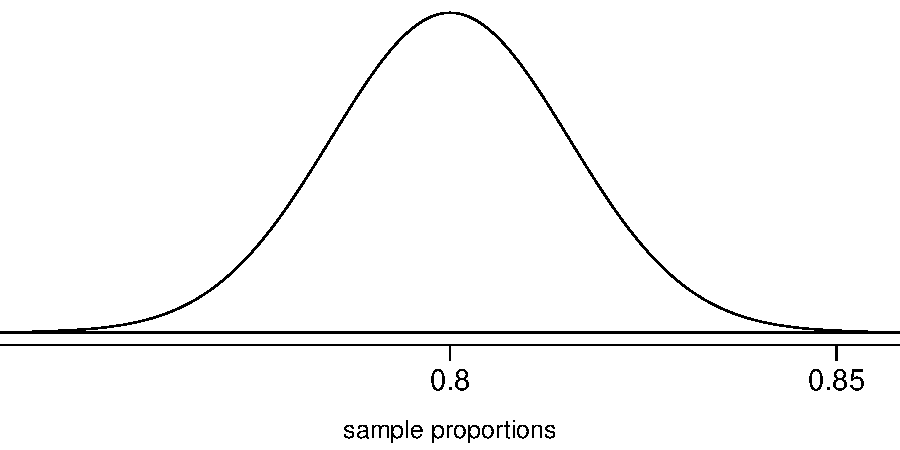
\includegraphics[width=\textwidth]{6-1_single_prop/figures/expdesgn_norm}
\end{center}
}
\pause
Since the p-value is low, we reject $H_0$. The data provide convincing evidence that more than 80\% of Americans have a good intuition on experimental design.

\end{frame}

%%%%%%%%%%%%%%%%%%%%%%%%%%%%%%%%%%%

\subsection{Recap}

%%%%%%%%%%%%%%%%%%%%%%%%%%%%%%%%%%%

\begin{frame}
\frametitle{}

\pq{11\% of 1,001 Americans responding to a 2006 Gallup survey stated that they have objections to celebrating Halloween on religious grounds. At 95\% confidence level, the margin of error for this survey is $\pm 3\%$. A news piece on this study's findings states: ``More than 10\% of all Americans have objections on religious grounds to celebrating Halloween." At 95\% confidence level, is this news piece's statement justified?}

\begin{enumerate}[(a)]
\item Yes
\solnMult{No}
\item Cannot tell
\end{enumerate}

\end{frame}

%%%%%%%%%%%%%%%%%%%%%%%%%%%%%%%%%%

\begin{frame}
\frametitle{Recap - inference for one proportion}

\begin{itemize}

\item Population parameter: $p$, point estimate: $\hat{p}$

\pause

\item Conditions:
\begin{itemize}
\item independence \\
- random sample and 10\% condition
\item at least 10 successes and failures\\ - if not $\rightarrow$ randomization
\end{itemize}

\pause

\item Standard error: $SE = \sqrt{ \frac{p(1-p)}{n} }$
\begin{itemize}
\item for CI: use $\hat{p}$
\item for HT: use $p_0$
\end{itemize}

\end{itemize}

\end{frame}